% ex24_fig1.tex
\begin{figure}[h]
	\begin{center}
	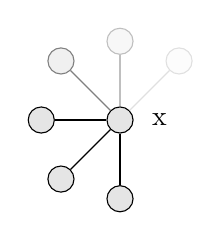
\begin{tikzpicture}
		\node[circle,draw,fill=black!10] (v) at (0,0) {};
		\node[] (vl) at (0.5,0) {x};
		\node[circle,draw,fill=black!10] (v2) at (-1,0) {}
			edge[-] (v);
		\node[circle,draw,fill=black!10] (v3) at (-0.75,-0.75) {}
			edge[-] (v);
		\node[circle,draw,fill=black!10] (v4) at (0,-1) {}
			edge[-] (v);
		\node[circle,draw=black!50,fill=black!6] (v5) at (-0.75,0.75) {}
			edge[-,draw=black!50] (v);
		\node[circle,draw=black!25,fill=black!3] (v6) at (0,1) {}
			edge[-,draw=black!25] (v);
		\node[circle,draw=black!12,fill=black!1] (v7) at (0.75,0.75) {}
			edge[-,draw=black!12] (v);
	\end{tikzpicture}
	\end{center}
	\caption{Exemple pour $k = 1$}
	\label{ex24_fig1}
\end{figure}

